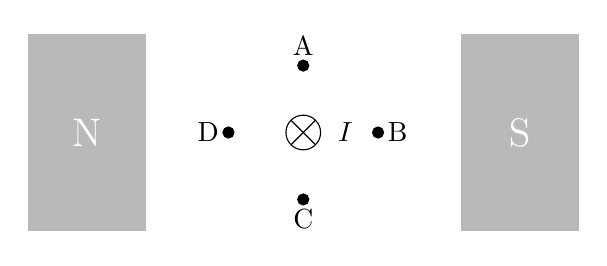
\begin{tikzpicture}
% N pole
\fill[gray!55] (-3.5,-1) rectangle (-2,1.5);
\node[white] at (-2.75,0.25) {\Large N};
% S pole
\fill[gray!55] (2,-1) rectangle (3.5,1.5);
\node[white] at (2.75,0.25) {\Large S};
% current into page
\draw (0,0.25) circle (0.22);
\draw (-0.155,0.405) -- (0.155,0.095);
\draw (-0.155,0.095) -- (0.155,0.405);
\node[right] at (0.32,0.25) {$I$};
% surrounding points
\filldraw (0,1.1) circle (2pt); \node[above] at (0,1.1) {A};
\filldraw (0.95,0.25) circle (2pt); \node[right] at (0.95,0.25) {B};
\filldraw (0,-0.6) circle (2pt); \node[below] at (0,-0.6) {C};
\filldraw (-0.95,0.25) circle (2pt); \node[left] at (-0.95,0.25) {D};
\end{tikzpicture}
